\documentclass{ctexart}
\usepackage{graphicx}
\graphicspath{{images/}}
\usepackage[backend=biber,style=gb7714-2015]{biblatex}
\addbibresource[location=local]{refer.bib}	
\title{中医治未病理论的社区“知信行”调查}
\author{付裕刚}
\date{\today}
\begin{document}
	\maketitle
	\begin{abstract}
	改革开放以来,随着经济条件的改善,人们开始注意到身心健康是生活安逸的重要保障,但是与此同时市场上养生保健方法鱼目混珠,一方面这些方法不够理论化、体系化,发挥作用寥寥;另一方面有的方法违背客观事实,有人甚至夸大作用,以此来谋求不当之财,污名化中医养生的应有作用。对于此类情景,我们应当正本清源,普及系统化科学的治未病理论,使它得以在新的时代发挥应有的活力,指导人们合适的生活调节方式,为新时期的预防保健工作做出系统性的贡献。为此,本次调查以南京市社区为样本采集点,致力于对当前人们对于中医治未病理论的认知、信念以及行动意愿,简称为“知信行”调查,为后面中医治未病理论的传播工作开展做一个描述性的统计分析。
	\end{abstract}
\tableofcontents
\section{项目流程设计}
对于该项目,主要流程有四个分支,分别是治未病理论支撑、治未病在社区卫生建设的应用、问卷设计和实际调研。本项目旨在将治未病理论依照知信行模式应用于社区的卫生保健上以提高居民的健康水平。

因此理论设计中医治未病理论、卫生保健制度和知信行模式。之后就是探讨治未病相关的内容哪些可以和社区卫生保健建设相结合,可以分为内容上的,形式上的,政策支持后的实施情况等等。在这方面还特别需要对人群进行区分,健康群体/疾病人群;年轻受众/老年受众等等的差异可能让这些方面的差异变得很大。

接下来是设计问卷的阶段,由中医专业的同学完成初步的条目设计,以及参照陈建伟对于中医社区调查的研究。然后提交给相关的专家老师进行筛选,结合老师给出的筛查建议来确定最终的条目。

接下来是实际调研阶段,预计在暑假完成,两个月的时间,主要是发放问卷,之后经过一段时间的间隔,做一次重测也是够的。如果时间紧还可以在开学后接着完成。调研方式是发放问卷,为了追踪调查对象的情况,应该是挨家挨户的拜访,还可以就部分人群抽样做一些访谈以积累更多的调研资料。

其中一个问题是社区的选取,应该遵循随机分布的原则。另外,江宁区有中医药特色社区,可以选为对照组。这样其他的社区作为空白组,来进行结果上的对比。之后和社区方面联系来确认最后的有效率的发放方式。

最后就是分析收集来的数据,完成论文阶段最后的写作。对于挑战杯而言还涉及各种展示等等,对于各个环节都应该拍摄相关的照片和做好相应的记录,以便于答辩的进行。
\begin{figure}[th]
	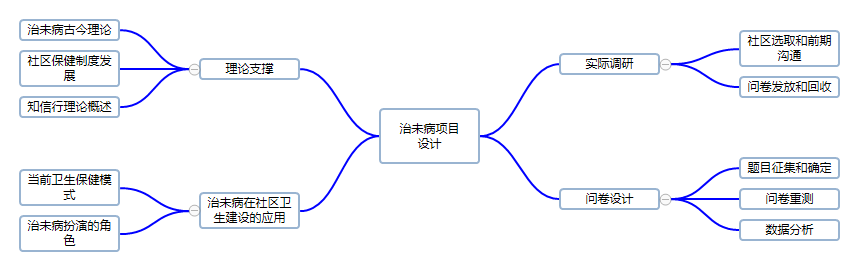
\includegraphics[width=\textwidth]{process.png}
	\centering
	\caption{项目设计简图}
\end{figure}
\section{治未病理论概述}
治未病是几千年来中国人在集体生活实践中发展而来的一种保持身体调达、心理安康的理论和实践方法。它基于一种忧患意识,表达了人们对于健康生活的渴望。随着时代的进步,治未病理论体系建立、发展、丰富,围绕理论逐步形成了一种有效的实践体系。治未病理论在总的原则上符合“三因制宜”,分别为顺应节气、符合地域、适应个人等三个层次,在具体的操作方法上有饮食调理、运动调理、精神调理等多种手段。

\subsection{治未病理论的历史溯源}
关于治未病的最早记载出现在《黄帝内经》之中,主要提出了未病先防和既病防变两个方面,为治未病理论提供了最初的理论框架。《素问·四气调神大论》曰:“圣人不治已病治未病,不治已乱治未乱,此之谓也。夫病已成而后药之,乱已成而后治之,譬犹渴而穿井,斗而铸锥,不亦晚乎!”\cite{南京中医学院医经教研组1981黄帝内经素问译释},说明养生的关键在于未病先防。《素问·阴阳应象大论》云 :“故邪风之至,疾如风雨 ,故善治者治皮毛,其次治肌肤,其次治筋脉, 其次治六腑, 其次治五脏 。治五脏者,半死半生也。”\cite{南京中医学院医经教研组1981黄帝内经素问译释},说明早期诊治可以得到更好的疗效,如果病邪已深,则治疗的预后不良。

后世的医家对《内经》提出的这一体系不断丰富,在历代医家的书籍中皆有论述。比如汉代的张仲景提出了六经辨证的体系,说明了疾病在脏腑之间的传变关系,提倡早期治疗,防微杜渐。唐代孙思邈则提出了“上医医未病之病,中医医欲病之病,下医医已病之病”\cite{李俊德2008中医必读百部名著}的说法,这一说法如今广为人知,可见防病、防变的思想影响深远。元代医家朱震亨在《格致余论》中提出:“与其求疗于有病之后,不若摄养于无疾之先;盖疾成而后药者,徒劳而已,……,未病而先治,所以明摄生之理。"\cite{朱震亨2008格致余论}清代名医叶天士在温病论治方面发展出卫气营血理论,揭示了外感温热病由表入里、由浅入深的一般规律,是对既病防变的又一重要补充。另外叶天士本人对于”未病先防“极为重视,他在《温热论》中指出:“务在先安未受邪之地。”\cite{叶桂2007温热论}

到了近现代,治未病理论体系得到了新的补充,主要体现在”欲病先防“和”病后防复“两个方面。现代人由于生活节奏紧张、精神压力大、饮食起居无节等因素,往往处于一种亚健康状态。这种状态往往持续时间长,无明显的疾病表观,但是此时正气不充,容易为外邪牵动内因而发病,处于”即将生病”的趋势之中,因而对于此类易感人群应该和健康的人群有所区分,由原先的“未病先防”转为“欲病先防”。而病后防复分为两个方面,其一是宋为民在其《未病论》\cite{宋为民1992未病论}中指出的“潜病未病态”,也就是对于季节性发作的疾病,例如慢性支气管炎在未发作时人的状态。而对于这样的疾病,“冬病夏治”是很好的办法,以防来年病情的反复或加重。其二是对于大病初愈之人,特别是恢复速度不快的儿童、老人等群体,应当嘱托其饮食起居上的注意,以防“食复”、“劳复”、“再受外邪而并发”等等。

\subsection{治未病理论的三个层次}
治未病理论在根本上离不开中医学的特色,一是以阴阳为根本进行调节以恢复人体的平衡,所谓“阴平阳秘,精神乃治”;二是天人合一下的整体观念,《灵枢·岁露》曰:“人与天地相参也,与日月相应也。“,揭示出人的生命活动与自然息息相关。在这样的大原则的指导下,治未病理论发展出和周围的环境相互协调的三个具体原则。
\begin{enumerate}
\item 顺应节气:《素问·四气调神大论》曰:“夫四时阴阳者,万物之根本也,所以圣人春夏养阳,秋冬养阴,以从其根。”\cite{南京中医学院医经教研组1981黄帝内经素问译释}古时以农耕文化为主体,人以四时节律为行为准则,以一天为周期看则“日出而作,日落而归”,以一年为周期看则“春种秋收”,具体农事活动又有二十四节气的指导。这样的顺应节气的思想在治未病理论当中也有相关的体现。以春季为例,《素问·四气调神大论》曰“春三月,此谓发陈,天地俱生,万物以荣,夜卧早起,广步于庭,被发缓形,以使志生,生而勿杀,予而勿夺,赏而勿罚,此春气之应,养生之道也。逆之则伤肝,夏为寒变,奉长者少。”\cite{南京中医学院医经教研组1981黄帝内经素问译释},可见自然节律和人养生防病是密切相关的,人应因时而动。

\item 符合地域:俗话说一方水土养一方人,我国幅员辽阔,地形复杂,生态环境多样。地理环境的差异造就了不同地域之中人体质、生活方式等等方面的差异。《灵枢·阴阳二十五人》根据人体各方面的特征进行系统分类,认为方位和五行相符,例如东方之人似木形人,尽管如今看来不够科学,但是表示古人已经认识到了不同地域之间人体的差异。《素问·五常政大论》指出“一州之气,生化寿夭不同……,高下之理,地势使然也。”\cite{南京中医学院医经教研组1981黄帝内经素问译释}也说明了水土不同对于人的寿命的影响。治未病也要考虑所在地域的特点,这一点也在实践中得到证实。例如四川地区喜爱食用折耳根,能够清除湿热,和四川地势较低,气候湿热的特征相符合,是饮食防病的良好实践。

\item 适应个人:人生来禀赋不同,体质有殊。王琦教授在既往体质分类研究的基础上 ,进一步完善了体质分类系统 ,将人体体质分为平和质、阴虚质、阳虚质、
阳盛质、气虚质、瘀血质、痰湿质、湿热质、气郁质9种基本中医体质类型\cite{王琦20059},为治未病提供了更加个性化的分类基础。治未病在实际操作中也需要依从个人实际情况制定相应的合理方案,不可一概而论以免伤身,违背了保全身体的初衷。
\end{enumerate}
\subsection{治未病理论的实践手段}
\begin{itemize}
\item 饮食调理:饮食调理指运用治未病理论中的饮食养生理论构建合理的膳食结构。人以五谷为养,合理的日常饮食和人的身体健康密切相关。治未病《素问·藏气法时论》提出“五谷为养,五果为助,五畜为益,五菜为充”。五谷、五果、五畜、五菜泛指各种谷物瓜果、肉类蔬菜,核心即为膳食平衡。这一理念在当前菜品逐渐丰富的情况下显得尤为重要:“高粱之变,足生大丁”,现代人喜欢流连于肥甘厚味的食肆,呼朋引伴推杯换盏之间人的健康就逐渐受损,长此以往五脏失调,疾病百生。

因此不论是对于身体健康的人,还是已经受损,处于亚健康状态或病后状态的人群而言,治未病理论能提供合理的理论支持,帮助人们回复膳食平衡。主要是对饮食种类的选择有所偏好,遵循五味调和的原则选取食物,并且适应一个人所处的年龄、体质、地域等等。
\item 运动调理:运动调理指借助特定的锻炼方法来达到活动筋骨、调畅气血,保持生命平衡的作用。《格致余论》云:“天之为物,故恒于动,人之有生亦恒于动”。治未病理论重视运动对于防治疾病的重要性,也为此发明出很多运动调理的方法。最早《内经》就提出练习气功来保全身体、防治疾病。东汉名医华佗依据导引术发明“五禽戏”,模仿动物姿态,效法自然来达到养生防病的目的。同样,一直为中老年群体喜爱的简化太极也因其动作和缓,张弛有度,能够调理呼吸、流通气血得到了群众的肯定。对于病后的人群,则遵医嘱进行适当的运动,也利于病后恢复。

\item 精神调理:精神调理指在治未病理论的指导下疏导情绪,保持心情调达和舒畅。
世卫组织已经提出健康的概念不仅指身体的健康,还有情志状态健康以及适应社会。中医极其重视人的精神情志的平衡状态,《内经·上古天真论》提出,“恬淡虚无,真气从之,精神内守,病安从来。”在当前竞争性的社会背景下,人们的生活受到来自学习、工作、人际交往等多个来源的压力。如果不能妥当处理好自身的情绪,就容易陷入“亚健康”状态,受到精神不振,情绪低落,反应迟钝和慢性病等等困扰。

因而掌握一些常见的疏导情绪的食材、药材配伍对于人的精神健康非常重要,特别是肝气理论擅于调节人的情志,辅以人的自主调节,在新时代有广泛的应用前景。
\end{itemize}
\section{知信行理论模式简介及其应用}
人们已经知道,在知识、信念和行为之间存在着一条沟壑:例如吸烟者知道吸烟存在的健康风险,即使他们了解后秉持了这一信念,他们却很难戒除吸烟的行为。在治未病理论的传播过程中,我们希望受众不仅仅是习得普遍的客体的知识,还能对此形成内化的信念并且真正地把这些知识应用于指导自身的生活。

在众多的理论模型中,知信行理论模式是应用最为广泛的模型,阐释了人的知识增长可以促进信念的加深进而转变为人的行为。知信行理论模式是认知理论和动机理论等在教育中的应用,主要探究了知识、信念和行为三者之前的联系。其中,知识是基础,信念(态度)是动力,行为则是目标。\cite{黄敬亨2006健康教育学}

“知”是某些明确的、得到普遍承认的客体知识。在知信行模式中,”知“代表通过某些媒介来传播知识,从而让人们“认知”和分析对象。“信”是在认识的基础上树立健康的“态度和信念”。“行”是在健康意志的指导下转变行为或养成行为习惯。\cite{金新政2003}

基于此模式进行的对照组研究在护理医学、预防医学领域形成了一套相对完备的体系,例如应用于糖尿病、高血压、呼吸系统慢性疾病的患者院外自理,术后康复,常见疾病预防等等。通过知信行模式,患者的院外自理能力加强,生活质量得到了提高,有的患者通过这一教育模式还形成了新的适应自身特点的生活模式。但是,知信行模式在治未病知识传播和实践当中的应用尚且缺乏,这也为我们的研究提供了创新的前景和空间。
\section{当前社区健康体系建设}
\subsection{社区和社区卫生服务的定义}
\subsubsection{社区}社会学家普遍认为一个社区应该包括一定数量的人口、一定范围的地域、一定规模的设施、一定特征的文化、一定类型的组织。换言之,社区是宏观社会的缩影,是聚居在一定地域范围内的人们所组成社会生活共同体。
\subsubsection{社区卫生服务}
社区卫生服务是社区服务中的一种最基本、普遍的服务,是由全科医生为主要卫生人力的卫生组织或机构所从事的一种社区定向的卫生服务,与医院定向的专科服务有所不同,它是社区建设的重要组成部分,以人的健康为中心、以家庭为单位、社区为范围、需求为导向,以妇女、儿童、老年人、慢性病患者、残疾人、低收入居民为重点,以解决社区主要卫生为题,满足基本医疗卫生服务需求为目的,融预防、医疗、保健、康复、健康教育和计划生育技术服务等为一体的,有效的、经济的、方便的、综合的、连续的基层卫生服务。 
\subsection{发展与现状}
从1985年的医疗卫生体制改革以来,“看病难、看病贵”的问题一直困扰着我国的医疗卫生体制。与西方成熟的社区医疗卫生模式相比,我国社区医疗起步较晚,于1996年开始试点,全面推动社区卫生服务体系的建设则在2000年开始进行。我国城市社区卫生服务的多年实践经验与国外社区卫生服务发展的成功经验告诉我们,发展社区卫生服务可以有效地解决居民“看病难、看病贵”的问题。一方面,发展社区卫生服务可以分流大医院的患者,解决居民“看病难”的问题,另一方面,社区卫生服务机构的预防保健、健康教育等服务可以有效提高居民自我保健意识,降低疾病发病率,同时,社区卫生服务机构提供的基本医疗服务价格比大医院低的多,可以在一定程度上降低居民的医疗支出,解决“看病贵”的问题。
\subsubsection{卫生资源分布不合理}
主要表现为卫生资源的分配比例和利用率的结构失衡。根据世界卫生组织的统计,社区卫生服务机构理应获得大部分的卫生资源。但是我国的情况正好相反:长期以来,在我国城市卫生服务工作中一直存在着重视综合型医疗卫生机构建设、轻视基层医疗卫生机构建设的情况。
\subsubsection{社区卫生服务补偿机制落实不足}
社区卫生服务的主要职责是向社区居民提供公共卫生服务和基本医疗服务,其本质是一项公益性的事业。社区卫生服务项目的开展需要政府在财政上给予充分的支持和保证。但目前我国政府对社区卫生服务机构的财政投入明显不足,社区医疗保险机构也没有将全部的社区卫生服务机构纳入医保定点机构,社区卫生服务机构的资金来源紧张,导致其难以有效地开展相关社区卫生服务项目。
\subsubsection{人力资源约束成社区卫生服务事业发展的瓶颈}
目前社区卫生服务机构中执业医生数量仅为综合性医院的4.5\%,且其中很多并不具有全科医生职业资格。公共卫生人员少,公共卫生的综合性技能差,预防和保健工作成为了社区卫生服务的弱项。因此,人才成为制约社区卫生服务发展的“瓶颈”。同时,全科医生培养模式不能适应社区卫生服务的发展要求,社区卫生服务机构的人力资源制度落后。
\subsubsection{缺少有效的监督机制}
鉴于我国医疗信息资源在医患之间严重不对称的现状,必须有一个监督主体的存在,对社区卫生服务机构的相关工作进行有效的监督。
\section{治未病理论在治未病社区健康建设的应用和前景}

\section{治未病“知信行”调查问卷的设计}
该问卷主要评价受调查者对中医治未病理论对于中医治未病理论的客观认知、所持信念以及行动意愿,以得出描述性的分析。设计的条目先进行征集,经编写后交付相关专家进行评议,并进行问卷重测以检验其信度。先前的研究有陈建伟对社区老年人进行的调查\cite{cjw_1_2009},其中拟定了一份“知信行”问卷可以进行部分参考。

\printbibliography
 \section{治未病问卷小样}
您好,这是一份由南京中医药大学第一临床医学院发起的调查问卷,旨在了解社区居民对于中医治未病理论的认知、行为等情况,响应“健康中国”工程,为后面中医治未病理论的传播做一个描述性统计分析。

本问卷时长约五分钟,我们郑重承诺,本问卷的所有数据仅用于科研用途,您的所有个人信息将受到相关法律的保护。

\begin{enumerate}
%知识部分
\item 中医学特点之一是整体观,认为“天人合一”,即人的健康受到周围环境(自然、社会、家庭)的影响。您认为:

A.正确\qquad B.部分正确\qquad C.错误 \qquad D.不清楚

\item 中医学认为人应该调节身体状况以适应气候、环境的变化。您认为:

A.正确\qquad B.部分正确\qquad C.错误 \qquad D.不清楚

\item 人的身体是一个整体,一个系统或器官的疾病可以影响其它系统或器官。您认为:

A.正确\qquad B.部分正确\qquad C.错误 \qquad D.不清楚

\item 人的情绪、精神状态对疾病有影响。您认为:

A.正确\qquad B.部分正确\qquad C.错误 \qquad D.不清楚

\item 人的健康与饮食有很大关系,中医的食疗指通过饮食调理来改变人的健康状况。
您认为:

A.正确\qquad B.部分正确\qquad C.错误 \qquad D.不清楚

\item 食物有寒凉等不同属性,人的体质也有阴阳等差别,所以饮食要根据体质不同进行选择。这个观点您认为:

A.正确\qquad B.部分正确\qquad C.错误 \qquad D.不清楚

\item 治未病理论认为“春夏养阳,秋冬养阴。”,因此夏天不要怕晒太阳,冬天不要大汗淋漓,这个观点您认为:

A.正确\qquad B.部分正确\qquad C.错误 \qquad D.不清楚

\item 刮痧、拔火罐、推拿等方法是治未病理论的运用,可以起到增强体质、保护健康的作用。这个说法您认为:

A.正确\qquad B.部分正确\qquad C.错误 \qquad D.不清楚

\item 各人的体质不同,所以他们应该根据自身的体质选择不同的饮食。这个说法您认为:

A.正确\qquad B.部分正确\qquad C.错误 \qquad D.不清楚

\item 有人说偏方也是是中医的一种,也能起到治病或保健的作用,您认为,

A.正确\qquad B.部分正确\qquad C.错误 \qquad D.不清楚

\item
草药煎汤服用是中医最常用的治疗方法,那么煎药时间越久越好,您认为,

A.正确\qquad B.部分正确\qquad C.错误 \qquad D.不清楚

\item 
治未病是中医特有的理论和方法,西医没有这样的说法,您认为,

A.正确\qquad B.部分正确\qquad C.错误 \qquad D.不清楚

\item 中医的存亡取决于中医的治疗是否有效,您认为,

A.正确\qquad B.部分正确\qquad C.错误 \qquad D.不清楚

%信念部分
\item 
您相信中医理论有其科学性,能从和西医不同的角度解释和解决疾病问题吗?

A.相信\qquad B.部分相信\qquad C.不相信\qquad D.不好说

\item 您本人能接受中医对您的诊断吗?

A.相信\qquad B.部分相信\qquad C.不相信\qquad D.不好说

\item 中医药的治疗(包括针灸、推拿、中药、中成药)只要选择得当,对治疗大多数疾病有效果,您相信吗?

A.相信\qquad B.部分相信\qquad C.不相信\qquad D.不好说

\item 您本人愿意接受中医药治疗方法吗?

A.愿意\qquad B.部分愿意\qquad C.不愿意 \qquad D.不好说

\item 您本人愿意尝试治未病提供的运动保健(太极拳、气功等)的方法吗?

A.愿意\qquad B.部分愿意\qquad C.不愿意 \qquad D.不好说

\item 您会用中医有关调畅情志的理论和方法来解决心理、情绪上的问题吗?

A.愿意\qquad B.部分愿意\qquad C.不愿意 \qquad D.不好说

\item 您愿意学习中医饮食调理的理论和方法并在日常饮食中加以运用吗?

A.愿意\qquad B.部分愿意\qquad C.不愿意 \qquad D.不好说

\item 
您对于当前国家出台政策,鼓励中医药发展怎么看?

A.我支持\qquad B.我保持中立\qquad C.我反对

\item 您喜欢看养生方面的书籍、视频等资料吗?

A.喜欢\qquad B.一般\qquad C.不喜欢\qquad D.我不清楚

%行为题目
\item
过去一年您接受中医治疗的次数?

A.0次 \qquad
B.1-2次\qquad
C.2-5次\qquad
D.5次以上

\item
您接受了哪一种中医治疗呢?

A.草药煎汤\qquad B.贴敷的膏药\qquad C.物理疗法,比如针灸,拔火罐等\qquad D.填写\underline{\makebox[6em]{}}

\item 您过去服用过几次膏方(固元膏、阿胶膏等等)吗?

A.0次\qquad B.1-2次\qquad C.3-5次\qquad D.5次以上

\item 您自己的孩子或者周围人的孩子接受过“三伏贴”来治疗肺部疾患吗?

A.有\qquad B.没有\qquad C.不清楚

\item 
您近一年来参加过几次养生知识的讲座?

A.0次\qquad B.1-2次\qquad C.3-5次\qquad D.5次以上

\item 
未来您会去接受中医治疗吗?

A.会\qquad B.不会\qquad C.可能

\item 
我们知道,电视台会播放中医节目,也有微信文章进行中医知识的传播。
\subitem 
   您收听/观看此类节目吗?
   
    A.从不\qquad B.偶尔\qquad C.经常

	\subitem 
    您阅读此类文章吗?
	
    A.从不\qquad B.偶尔\qquad C.经常
    
    \subitem 
    您会仿效节目/文章中的做法吗?
	
	A.从不\qquad B.偶尔\qquad C.经常
    
    \subitem 
   您能坚持节目/文章里面的做法吗?
   
    A.我能坚持做\qquad B.坚持不久就放弃了\qquad C.我没做过
    
\item 
您的
性别\underline{\makebox[6em]{}}
年龄\underline{\makebox[6em]{}}
学历\underline{\makebox[6em]{}}
年收入情况\underline{\makebox[6em]{}}
\newline
感谢您的参与以及对我们的支持!
\end{enumerate}

\end{document}